\scanpage{87}

\[
\begin{aligned}
&\unsure{z|\zeta|\xi}_1\quad z_{14}\quad z_4\quad z'_2\\
&z_1\,\big|\,z'_2\ z'_3\ z_{31}\ z_{12}
\end{aligned}
\]

\diagram{%
\begin{tikzcd}[ampersand replacement=\&,column sep=0pt,row sep=0pt]
|[inner sep=0pt]| \vcenter{\hbox{%
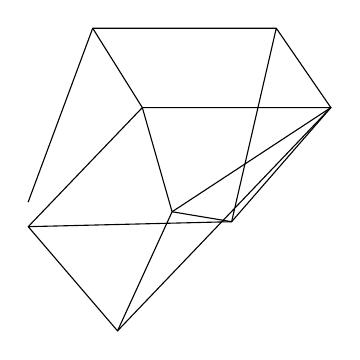
\begin{tikzpicture}[x=0.063cm,y=-0.063cm,line cap=round,line join=round,line width=.4pt]
\draw (0,36) -- (13,1) -- (50,1) -- (61,17) -- (18,62) -- (0,41) -- (41,40) -- (50,1);
\draw (13,1) -- (23,17) -- (61,17);
\draw (0,41) -- (23,17) -- (29,38) -- (61,17);
\draw (18,62) -- (29,38) -- (41,40) -- (61,17);
\end{tikzpicture}%
}}
\end{tikzcd}%
}

\diagram{%
\begin{tikzcd}[ampersand replacement=\&,column sep=0pt,row sep=0pt]
|[inner sep=0pt]| \vcenter{\hbox{%
\begin{tikzpicture}[x=0.066cm,y=-0.066cm,line cap=round,line join=round,line width=.4pt]
\draw[thick] (0,0) -- (0,18);
\draw (0,0) -- (26,18) -- (26,0);
\draw (1,22) -- (3,39);
\draw (26,21) -- (29,39);
\node[inner sep=.55pt,anchor=center,font=\scriptsize] at (-4,9) {$\delta$};
\node[inner sep=.55pt,anchor=center,font=\scriptsize] at (16,3) {$\delta'$};
\node[inner sep=.55pt,anchor=center,font=\scriptsize] at (34,8) {$\delta''$};
\node[inner sep=.55pt,anchor=center,font=\scriptsize] at (-6,30) {$\delta'''$};
\node[inner sep=.55pt,anchor=center,font=\scriptsize] at (35,27) {$\delta^{\mathrm{IV}}$};
\fill (48,2) circle[radius=0.0225cm];
\fill (52,18) circle[radius=0.0225cm];
\fill (52,39) circle[radius=0.0225cm];
\fill (65,8) circle[radius=0.0225cm];
\fill (65,18) circle[radius=0.0225cm];
\fill (65,39) circle[radius=0.0225cm];
\end{tikzpicture}%
}}
\end{tikzcd}%
}

\[
\begin{aligned}
\delta&=z_1,\quad\delta'=z_2,\quad\delta''=\unsure{z'_2|J'_2|\xi'_2}\\
\delta'''&=z_{14}\quad\delta^{\mathrm{IV}}=z_{25}
\end{aligned}\qquad
\begin{aligned}
\delta\delta'&=0&\delta\delta''&=1\\
\delta\delta'''&=1&\delta\delta^{\mathrm{IV}}&=0
\end{aligned}
\]

\diagram{%
\begin{tikzcd}[ampersand replacement=\&,column sep=0pt,row sep=0pt]
|[inner sep=0pt]| \vcenter{\hbox{%
\begin{tikzpicture}[x=0.06cm,y=-0.06cm,line cap=round,line join=round,line width=.4pt]
\draw (0,0) -- (0,24);
\fill (0,12) circle[radius=0.05cm];
\end{tikzpicture}%
}}
\end{tikzcd}%
}

\[
\delta\delta'\ \deleted{\bmod 2}\equiv\operatorname{card}(\delta\cap\delta')+\operatorname{card}(\varepsilon(\delta)\cap\varepsilon(\delta'))
\]

\diagram{%
\begin{tikzcd}[ampersand replacement=\&,column sep=0pt,row sep=0pt]
|[inner sep=0pt]| \vcenter{\hbox{%
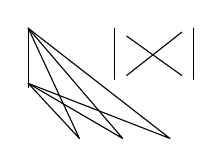
\begin{tikzpicture}[x=0.05cm,y=-0.05cm,line cap=round,line join=round,line width=.4pt]
\draw (0,0) -- (0,15);
\draw (0,0) -- (13,28) -- (0,14);
\draw (0,0) -- (24,28) -- (0,14);
\draw (0,0) -- (36,28) -- (0,14);
\draw (22,0) -- (22,13);
\draw (42,0) -- (42,13);
\draw (25,2) -- (39,12);
\draw (25,12) -- (39,1);
\end{tikzpicture}%
}}
\end{tikzcd}%
}

\diagram{%
\begin{tikzcd}[ampersand replacement=\&,column sep=0pt,row sep=0pt]
|[inner sep=0pt]| \vcenter{\hbox{%
\begin{tikzpicture}[x=0.05cm,y=-0.05cm,line cap=round,line join=round,line width=.4pt]
\draw (0,0) -- (1,14);
\draw (11,0) -- (12,14);
\draw (23,0) -- (23,29);
\draw (1,16) -- (-1,29) -- (2,27);
\draw (1,37) -- (1,46);
\end{tikzpicture}%
}}
\end{tikzcd}%
}

\diagram{%
\begin{tikzcd}[ampersand replacement=\&,column sep=0pt,row sep=0pt]
|[inner sep=0pt]| \vcenter{\hbox{%
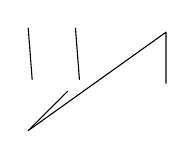
\begin{tikzpicture}[x=0.05cm,y=-0.05cm,line cap=round,line join=round,line width=.4pt]
\draw (0,0) -- (1,13);
\draw (12,0) -- (13,13);
\draw (0,26) -- (35,1) -- (35,14);
\draw (0,26) -- (10,16);
\end{tikzpicture}%
}}
\end{tikzcd}%
}

\diagram{%
\begin{tikzcd}[ampersand replacement=\&,column sep=0pt,row sep=0pt]
|[inner sep=0pt]| \vcenter{\hbox{%
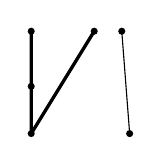
\begin{tikzpicture}[x=0.05cm,y=-0.05cm,line cap=round,line join=round,line width=.4pt]
\draw[very thick] (0,0) -- (0,26) -- (16,0);
\draw (23,0) -- (25,26);
\fill (0,0) circle[radius=0.045cm];
\fill (0,14) circle[radius=0.045cm];
\fill (0,26) circle[radius=0.045cm];
\fill (16,0) circle[radius=0.045cm];
\fill (23,0) circle[radius=0.045cm];
\fill (25,26) circle[radius=0.045cm];
\end{tikzpicture}%
}}
\end{tikzcd}%
}

\diagram{%
\begin{tikzcd}[ampersand replacement=\&,column sep=0pt,row sep=0pt]
|[inner sep=0pt]| \vcenter{\hbox{%
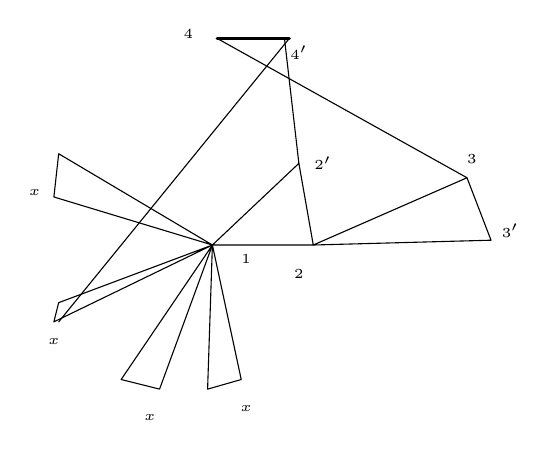
\begin{tikzpicture}[x=0.061cm,y=-0.061cm,line cap=round,line join=round,line width=.4pt]
\draw (33,44) -- (0,34) -- (1,25) -- cycle;
\draw (33,44) -- (0,60) -- (1,56) -- cycle;
\draw (33,44) -- (14,72) -- (22,74) -- cycle;
\draw (33,44) -- (32,74) -- (39,72) -- cycle;
\draw (33,44) -- (54,44) -- (51,27) -- cycle;
\draw (54,44) -- (86,30) -- (91,43) -- cycle;
\draw (1,60) -- (49,1) -- (34,1) -- (86,30);
\draw[very thick] (34,1) -- (49,1);
\draw (48,1) -- (51,27);
\node[inner sep=.55pt,anchor=center,font=\tiny] at (-4,33) {$x$};
\node[inner sep=.55pt,anchor=center,font=\tiny] at (0,64) {$x$};
\node[inner sep=.55pt,anchor=center,font=\tiny] at (20,80) {$x$};
\node[inner sep=.55pt,anchor=center,font=\tiny] at (40,78) {$x$};
\node[inner sep=.55pt,anchor=center,font=\tiny] at (40,47) {$1$};
\node[inner sep=.55pt,anchor=center,font=\tiny] at (51,50) {$2$};
\node[inner sep=.55pt,anchor=center,font=\tiny] at (56,27) {$2'$};
\node[inner sep=.55pt,anchor=center,font=\tiny] at (87,26) {$3$};
\node[inner sep=.55pt,anchor=center,font=\tiny] at (95,41) {$3'$};
\node[inner sep=.55pt,anchor=center,font=\tiny] at (28,0) {$4$};
\node[inner sep=.55pt,anchor=center,font=\tiny] at (51,4) {$\unsure{4'}$};
\end{tikzpicture}%
}}
\end{tikzcd}%
}

\unsure{hexagone|hexagones} pointés orientés

\[
\underbrace{27}\cdot10\cdot\underbrace{8\cdot4}\cdot1\cdot\underbrace{1}
=2^6\cdot3^{\unsure{3|2}}\cdot5=[W]:6
\]

hexagones : $[W]:72$

\diagram{%
\begin{tikzcd}[ampersand replacement=\&,column sep=0pt,row sep=0pt]
|[inner sep=0pt]| \vcenter{\hbox{%
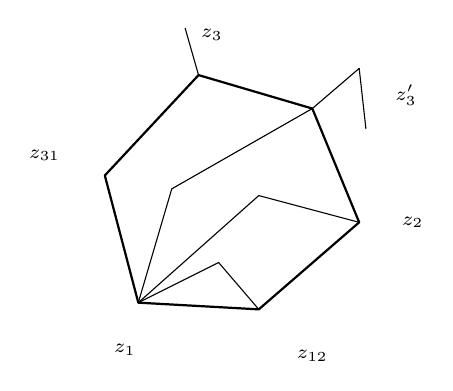
\begin{tikzpicture}[x=0.085cm,y=-0.085cm,line cap=round,line join=round,line width=.4pt]
\draw[thick] (0,22) -- (14,7) -- (31,12) -- (38,29) -- (23,42) -- (5,41) -- cycle;
\draw (14,7) -- (12,0);
\draw (31,12) -- (38,6) -- (39,15);
\draw (5,41) -- (10,24) -- (31,12);
\draw (5,41) -- (23,25) -- (38,29);
\draw (5,41) -- (17,35) -- (23,42);
\node[inner sep=.55pt,anchor=center,font=\scriptsize] at (-9,19) {$z_{31}$};
\node[inner sep=.55pt,anchor=center,font=\scriptsize] at (16,1) {$z_3$};
\node[inner sep=.55pt,anchor=center,font=\scriptsize] at (45,10) {$z'_3$};
\node[inner sep=.55pt,anchor=center,font=\scriptsize] at (46,29) {$z_2$};
\node[inner sep=.55pt,anchor=center,font=\scriptsize] at (31,49) {$z_{12}$};
\node[inner sep=.55pt,anchor=center,font=\scriptsize] at (3,48) {$z_1$};
\end{tikzpicture}%
}}
\end{tikzcd}%
}

\diagram{%
\begin{tikzcd}[ampersand replacement=\&,column sep=0pt,row sep=0pt]
|[inner sep=0pt]| \vcenter{\hbox{%
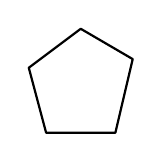
\begin{tikzpicture}[x=0.055cm,y=-0.055cm,line cap=round,line join=round,line width=.4pt]
\draw[thick] (0,9) -- (12,0) -- (24,7) -- (20,24) -- (4,24) -- cycle;
\end{tikzpicture}%
}}
\end{tikzcd}%
}

pentagones pointés orientés

\[27\cdot10\cdot8\cdot4\cdot3\overset{\displaystyle=2^6 3^4 5}{=}[W]:2\]

pentagones \quad $[W]:20$

\[
\begin{aligned}
\text{\unsure{carré|carrés} pointés}\quad&27\cdot10\cdot8\cdot4=[W]:6\\
\text{carrés}:&\ [W]:48
\end{aligned}
\]

\[\mathbb F_2^{\unsure{4|i}}\quad\vert\]

\diagram{%
\begin{tikzcd}[ampersand replacement=\&,column sep=0pt,row sep=0pt]
|[inner sep=0pt]| \vcenter{\hbox{%
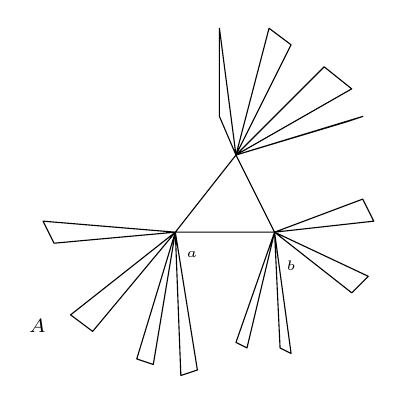
\begin{tikzpicture}[x=0.07cm,y=-0.07cm,line cap=round,line join=round,line width=.4pt]
\draw (15,28) -- (33,28) -- (26,14) -- cycle;
\draw (26,14) -- (23,-9) -- (23,7) -- cycle;
\draw (26,14) -- (32,-9) -- (36,-6) -- cycle;
\draw (26,14) -- (42,-2) -- (47,2) -- cycle;
\draw (26,14) -- (46,8) -- (49,7) -- cycle;
\draw (15,28) -- (-9,26) -- (-7,30) -- cycle;
\draw (15,28) -- (-4,43) -- (0,46) -- cycle;
\draw (15,28) -- (8,51) -- (11,52) -- cycle;
\draw (15,28) -- (16,54) -- (19,53) -- cycle;
\draw (33,28) -- (51,26) -- (49,22) -- cycle;
\draw (33,28) -- (47,39) -- (50,36) -- cycle;
\draw (33,28) -- (34,49) -- (36,50) -- cycle;
\draw (33,28) -- (26,48) -- (28,49) -- cycle;
\node[inner sep=.55pt,anchor=center,font=\scriptsize] at (-10,45) {$A$};
\node[inner sep=.55pt,anchor=center,font=\tiny] at (18,32) {$a$};
\node[inner sep=.55pt,anchor=center,font=\tiny] at (36,34) {$b$};
\end{tikzpicture}%
}}
\end{tikzcd}%
}

\[
\text{\unsure{Calculons|Combien|Conditions}\ \operatorname{card}}\quad |\{z\in\widetilde A\quad\text{\unsure{z lié à x.|$\xi$ liés à $x$}}\]
\[\lambda_{12}\quad\lambda_{23}\quad\lambda_{4\unsure{\cdot}}\]

\[
\begin{aligned}
\mathbb F_2^A&\ \mathrm P\\[-2pt]
&x,y\qquad x-y=u\in\mathbb F_2^A\simeq\mathscr P(A)
\end{aligned}
\]

former les $\alpha\in A$ sur lesquels $\operatorname{Et}(x)\cap\widetilde A$ \inserted{et $\operatorname{Et}(y)\cap\widetilde A$} \deleted{\unsure{coïncident}} sont distincts

\[
x,y\ \text{liés}\Longleftrightarrow
\left\{\begin{aligned}
&x\text{ et }y\text{ de même parité},\quad \text{i.e. card }u\text{ paire}:\\
&\quad x-y=\mathbf1\ \unsure{=A|{}^{A}}\quad
 (\operatorname{Et}(x)\cap\widetilde A\text{ et }\operatorname{Et}(y)\cap\widetilde A\text{ sont complémentaires})\\
&\text{\unsure{pour}}\quad x\text{ et }y\text{ de parité }\unsure{\ne|\text{contr.}},\quad\text{i.e. card }u\text{ impaire}:\\
&\quad\deleted{\unsure{x-y}}\quad \underline{\operatorname{card}u=3}
\end{aligned}\right.
\]

\[
\underline{x,y\ \text{non liés}}\Longleftrightarrow
\left\{\begin{aligned}
&x\text{ et }y\text{ de même parité i.e. card }u\text{ paire}:\quad x-y\ne\mathbf 1\\
&\quad\text{i.e. }(\operatorname{Et}(x)\cap\widetilde A)\cap\operatorname{Et}(y)\cap\widetilde A\ne\varnothing\\
&x\text{ et }y\text{ de parité contr.}:\quad\operatorname{card}u=1\\
&\quad\text{i.e. card }u\text{ impaire}
\end{aligned}\right.
\]

\diagram{%
\begin{tikzcd}[ampersand replacement=\&,column sep=0pt,row sep=0pt]
|[inner sep=0pt]| \vcenter{\hbox{%
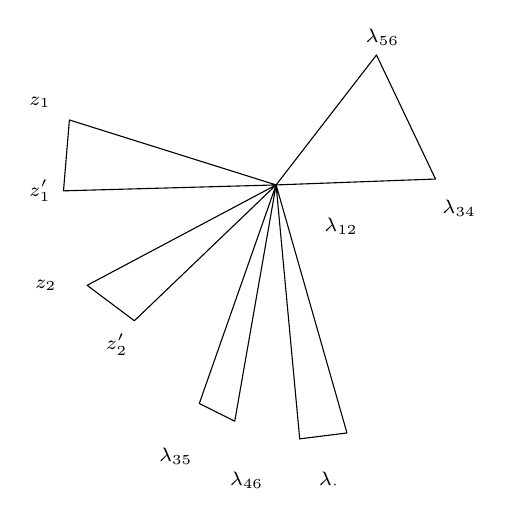
\begin{tikzpicture}[x=0.075cm,y=-0.075cm,line cap=round,line join=round,line width=.4pt]
\draw (35,22) -- (52,0) -- (62,21) -- cycle;
\draw (35,22) -- (0,11) -- (-1,23) -- cycle;
\draw (35,22) -- (3,39) -- (11,45) -- cycle;
\draw (35,22) -- (22,59) -- (28,62) -- cycle;
\draw (35,22) -- (39,65) -- (47,64) -- cycle;
\node[inner sep=.55pt,anchor=center,font=\scriptsize] at (53,-3) {$\lambda_{56}$};
\node[inner sep=.55pt,anchor=center,font=\scriptsize] at (66,26) {$\lambda_{34}$};
\node[inner sep=.55pt,anchor=center,font=\scriptsize] at (46,29) {$\lambda_{12}$};
\node[inner sep=.55pt,anchor=center,font=\scriptsize] at (-5,8) {$z_1$};
\node[inner sep=.55pt,anchor=center,font=\scriptsize] at (-5,23) {$z'_1$};
\node[inner sep=.55pt,anchor=center,font=\scriptsize] at (-4,39) {$z_2$};
\node[inner sep=.55pt,anchor=center,font=\scriptsize] at (8,49) {$z'_2$};
\node[inner sep=.55pt,anchor=center,font=\scriptsize] at (18,68) {$\lambda_{35}$};
\node[inner sep=.55pt,anchor=center,font=\scriptsize] at (30,72) {$\lambda_{46}$};
\node[inner sep=.55pt,anchor=center,font=\scriptsize] at (44,72) {$\lambda_{\unsure{\cdot}}$};
\end{tikzpicture}%
}}
\end{tikzcd}%
}

\[
\begin{aligned}
x,y\ \text{liés}&\Longleftrightarrow\operatorname{card}u=3\text{ ou }4\\
x,y\ \text{non liés}&\Longleftrightarrow\operatorname{card}u=\underset{(x=y)}{0},1\text{ ou }2
\end{aligned}
\]

\diagram{%
\begin{tikzcd}[ampersand replacement=\&,column sep=0pt,row sep=0pt]
|[inner sep=0pt]| \vcenter{\hbox{%
\begin{tikzpicture}[x=0.065cm,y=-0.065cm,line cap=round,line join=round,line width=.4pt]
\draw (9,0) -- (51,49);
\draw (0,8) -- (5,18);
\fill (5,18) circle[radius=0.0325cm];
\draw (10,23) -- (18,33);
\fill (18,33) circle[radius=0.0325cm];
\draw (22,36) -- (31,46);
\fill (31,46) circle[radius=0.0325cm];
\draw (35,50) -- (42,57);
\fill (42,57) circle[radius=0.0325cm];
\draw (18,0) -- (23,9);
\fill (23,9) circle[radius=0.0325cm];
\draw (27,15) -- (34,24);
\fill (34,24) circle[radius=0.0325cm];
\draw (39,29) -- (45,38);
\fill (45,38) circle[radius=0.0325cm];
\draw (50,43) -- (57,51);
\fill (57,51) circle[radius=0.0325cm];
\node[inner sep=.55pt,anchor=center,font=\tiny] at (0,8) {$+$};
\node[inner sep=.55pt,anchor=center,font=\tiny] at (18,33) {$+$};
\node[inner sep=.55pt,anchor=center,font=\tiny] at (31,46) {$+$};
\node[inner sep=.55pt,anchor=center,font=\tiny] at (42,57) {$+$};
\node[inner sep=.55pt,anchor=center,font=\tiny] at (18,0) {$+$};
\node[inner sep=.55pt,anchor=center,font=\tiny] at (34,24) {$+$};
\node[inner sep=.55pt,anchor=center,font=\tiny] at (45,38) {$+$};
\node[inner sep=.55pt,anchor=center,font=\tiny] at (57,51) {$+$};
\end{tikzpicture}%
}}
\end{tikzcd}%
}

\[
\begin{aligned}
\text{triangles pointés orientés}\quad&27\cdot10=270=[W]:\unsure{2^6\cdot3^1|2^3\cdot3^4}\\
\text{triangles}:\quad&\frac{27\cdot10}{6}=45=[W]:2^7\cdot3^2
\end{aligned}
\]

% archive sheet number: 86
